Before we describe $\mathcal{M} (K[T])$ it is useful to study $K$ as a topological/metric space first.
\subsection{The topology of $K$} \label{sec:ultrametric_spaces}

Recall that $K$ is a metric space with the metric $d(a, b) = |a - b|$. 
This metric satisfies a stronger version of the triangle inequality. 
Such metrics are known as ultrametrics. 
\begin{definition}
	A \emph{ultrametric space} is a topological spaces $(X, d)$ where the metric satisfies the non-archimedean triangle inequality. 
	\[
		d(x, y) \le \max \{d(x, z) ,d(z, y)\}, \quad \forall x, y ,z \in X
	.\] 
\end{definition}
\begin{lemma}
	If $d(x,z) \ne d(z,y)$ the inequality is an equality. 
\end{lemma}
\begin{proof}
	Suppose without loss of generality that $d(x, z) \ge d(z,y)$, so 
	\[	
		d(x, y) \le \max \{d(x, z), d(z,y)\} = d(x, z)
	.\] 
	Then $d(x, z) \le \max \{d(x, y), d(y,z)\}$. So $d(x, z) \le d(x, y) \le d(x, z)$. This proves equality.
\end{proof}
\begin{corollary}
	Balls/disks in ultra metric spaces have some unusual behavior
	\begin{itemize}
		\item Any point of a ball (open or closed) is a center for that ball. 
		\item Two balls are either disjoint, or one is contained in the other.  
	\end{itemize}
	See \cref{fig:oddities_of_ultrametric_balls}.
\end{corollary}
\begin{figure}[h]
    \centering
    \incfig{oddities-of-ultrametric-balls}
    \caption{Oddities of disks in ultrametric spaces}
    \label{fig:oddities_of_ultrametric_balls}
\end{figure}
\begin{corollary}
	The topology of $X$ is totally disconnected. 
\end{corollary}

\subsection{The Berkovich affine line when $K$ is algebraically closed} \label{sec:the_berkovich_affine_line}

We will describe the Berkovich space of the polynomials in one variable  $\mathcal{M} (K[T])$.
We first do this for $K$ algebraically closed, and the explain how to expand to the case where $K$ is discretely valued.
We call the resulting space $\aff_K^{1, \text{an}}$, the \emph{analytification of the affine line}, or sometimes the \emph{Berkovich affine line}. 

\medskip

One way to find norms on $K[T]$ would taking a point $a \in K$ and define $|f|_a = |f(a)|_K$ where $|\cdot |_K$ is the norm on $K$. 
So there is a natural embedding $K \into \mathcal{M}(K[T])$ and we will implicitly identify these points.  

Another way to define a norm is by choosing a closed disk $B(a, r) = \{x \in K \st |x - a| \le r\} $ with center $a$, and radius $r$ and define \[
	|f|_{B(a, r)} = \sup_{x \in B(a, r)} |f(x)|
.\] 
\begin{claim}
	The norm $|f|_{B(a, r)}$ as defined above is a well defined multiplicative seminorm extending the norm on $K$. 
	If $r \in |K|$ then the supremum is a maximum and the maximum is obtained for some point on the boundary of $B(a, r)$.
	Moreover, if  $f = \sum_{i = 0}^{n} b_i (T-a)^{i}$ is the Taylor expansion of $f$ around $a$ then for any $r \in [0, \infty)$ the norm can be computed as \begin{equation}\label{eq:norm_disk_taylor}
		|f|_{B(a, r)} = \max_{i}\{  |b_i|r^{i}\}
	.\end{equation} 
\end{claim}
\begin{proof}
	Let $f = \sum_{i = 0}^{n} a_i T^{i}$. 
	Then for $x \in B(a, r)$ we have $|x| \le |a| + r$. 
	So  $|f(x)| \le  \sum_{i = 0}^{n} |a_i| |x|^{i} \le \sum_{i = 0}^{n}|a_i| (|a| + r)^{i} $. 
	This last bound is independent of $x$. Hence the supremum exists. 

	Non-archimedean triangle inequality and extending the norm on $K$ is easily checked. 
	The multiplicatively is a little bit more subtle. 

	Without loss of generality we may translate the disk such that $a = 0$. 
	Lets assume for now that $r \in |K|$.
	Then we may also rescale such that $r = 1$. 

	Clearly the seminorm is multiplicative for elements in  $K$, i.e.\ for every $\lambda \in K, f \in K[t]: |\lambda \cdot f|_{B(a, r)} = |\lambda|\cdot |f|_{B(a, r)}$.  Let $f, g \in K[T]$, which we may rescale by an element of $K$, such that the largest coefficient of $f, g$ has norm $1$. In particular this means that $|f|_{B(0,1)}, |g|_{B(0,1)} \le 1$. 
	Then $f, g \in R[T]$ and their  reductions modulo  $\pi$ $\overline{f}, \overline{g} \in k[T]$ are nonzero.
	So $\overline{f}, \overline{g}$ have only a finite number of roots. In particular these is some $\overline{a} \in k$, represented by $a \in R$ such that $\overline{f}(\overline{a}) \ne 0, \overline{f}(\overline{a})\ne 0$. 
	So $f(a), g(a) \in R = B(0, 1)$ and $|f(a)| = |g(a)| = 1$. 
	In particular \cref{eq:norm_disk_taylor} holds. 
	So the supremum is obtained in $a$ for both polynomials and the norm is multiplicative as the supremem for $f\cdot g$ will also be obtained in $a$. 


	To obtain the result also holds for $r \not\in |K^{\times }|$, we use that any such disk $B(a, r)$ can be written as an increasing union of closed disks with radii in the value group. The result now follows from the continuity of \cref{eq:norm_disk_taylor} and the continuity of multiplication. 
\end{proof}



So the space of closed discs in $K$, which includes points (discs of radius zero), embeds as well in $\mathcal{M} (K[T])$. 
As we will see in a second these will make up almost all of the points on $\mathcal{M} (K[T])$. 
If we ignore these missing points for a moment, this means that $\mathcal{M}(K[T])$ is connected. 
Indeed, let $a \in K$ be any point. Then we can define a line \begin{equation}\label{eq:line_in_A_1}
	\ell_a: [0, \infty) \to  \aff_K^{1, \text{an}}: r\mapsto B(a, r)
\end{equation}
Because in an ultrametric space any point in a ball is a centre of ball, we see that for any two points $a, b$ the lines $\ell_a, \ell_b$ coincide for any $r \ge |a - b|$. 
So $\aff_K^{1,\text{an}}$ is not only connected, it is path connected!
This is illustrated in \cref{fig:the_lines_la_lb_lc}. 
\begin{figure}[h]
    \centering
    \incfig{the-lines-la-lb-lc}
    \caption{The lines $\ell_a, \ell_b, \ell_c$ join up (i.e.\ define the same disk) when the radious $r$ is greater than the distance between the points.}
    \label{fig:the_lines_la_lb_lc}
\end{figure}

We have been missing a few points on $\aff_K^{1, \text{an}}$. 
The Berkovich classification theorem gives all points. 
\begin{theorem}
	[Berkovich classification theorem, \cite{bakerarizona}] \label{thm:berkovich_classification}
	Assume that $K$ is algebraically closed. 
	Any point $x \in \aff_K^{1,\text{an}}$ is given by a decreasing sequences of closed disks $B_n = B(a_n, r_n)$ in $K$ by the formula \begin{equation}\label{eq:norm_disk_polynomial}
	|f|_x = \lim_{n \to \infty} |f|_{B_n}
	.\end{equation}
	Moreover, two such sequences $B_n, B'_n$ define the same norm if and only if:
	 \begin{itemize}
		\item Both sequences have the same non-emtpy intersection, i.e.\ $\bigcap_{n = 1}^{\infty} B_n = \bigcap_{n = 1}^{\infty} B_n' \ne \emptyset$. 
			In this case the intersection $B = \bigcap_{n \in N} B_n$ is a closed disk (possibly a point) and $x = |\cdot |_B$. 
		\item Both sequences have empty intersection, i.e.\ $\bigcap_{n = 1}^{\infty} B_n = \bigcap_{n = 1}^{\infty} B_n' = \emptyset$  and for every $n$ there is an $m$ such that $B'_m \subset  B_n$  and $B_m \subset  B'_n$.
	\end{itemize}
	This means that we can classify the points in $\aff ^{1,\text{an}}_K$ into four types depending on $B = \bigcap_{n \in \N} B_n$. 
	\begin{description}
		\item[Type 1:] $B = \{a\} $ a point and the $|f|_x = |f(a)|$. 
		\item[Type 2:] $B = B(a, r)$ with $r \in |K^* |$ and $|f|_x = |f|_{B(a, r)}$
		\item[Type 3:] $B = B (a, r)$ with $r \not\in |K^*|$ and $|f|_x = |f|_{B(a, r)}$
		\item[Type 4:] $B = \emptyset$
	\end{description}
\end{theorem}
As we can see our previous discussion has excluded type four points. We will see an example of such point in \cref{ex:type4point}. 

\begin{proof}
	I will only show the proof that every norm is given by such a sequence as the proofs of all other statements are technical and give little insight. 

	Let $x \in \aff_K^{1, \text{an}}$ be a multiplicative seminorm on $K[T]$. 
	As  $K$ is algebraically closed every polynomial factors into linear factors $(T-a)$. 
	Hence $x$ is uniquely determined by its value $|T-a|_x$ for each $a \in K$. 
	We will write $\rho_a = |T-a|_x$.
	Let  $a, b \in K$ such that $\rho_a \le \rho_b$. 
	Then  \begin{equation}\label{eq:proof_berk_class_1}
		|a - b|_x = |(T-b) - (T - a)|_x \le \max \{\rho_a, \rho_b\} = \rho_b 
	.\end{equation} 
	Hence $a \in B_{b, \rho_b}$ and thus  $B(a, \rho_a) \subseteq B(b, \rho_b)$. 

	Define $\rho := \inf_{a \in K} \rho_a$ and let $a_1, a_2, \ldots$ be a sequence such that $(\rho_{a_i})_{i \in \N}  $ is a non-increasing sequence converging to $\rho$. 
	By the previous remark this gives a decreasing sequence of disks \[
		B(a_1, \rho_{a_1}) \supset B(a_2, \rho_{a_2}) \supset B(a_3, \rho_{a_3}) \supset\ldots
	.\] 
	Now we will check that $|\cdot |_x = \lim_{n \to \infty} |\cdot |_{B(a_i, \rho_i)}$ by verifying that both norms agree on $T- b$ for every $b \in K$. 
	 There are two cases. Either $|T - b|_x = \rho_b = \rho$ or $\rho_b \ge \rho_{a_i}$ for some $i$. 

	 If $ \rho_b = \rho$ then by \eqref{eq:proof_berk_class_1} we find $|b - a_i|_x \le \rho_n$ for all $i$.
	 So \[
		 |T - b|_{B(a_i, \rho_i)} = |(T - a_i) - (b_i - a_i)|_{B(a_i, \rho_i)} = \max(\rho_n, |b - a_i|) = \rho_n
	 .\]
	 So $\lim_{i \to \infty} |T- b|_{B(a_i, \rho_i)} = \rho = |T - b|$. 

	 If $\rho_b > \rho$ then for $n \gg 0$ we have $\rho_b > \rho_a$ and thus $|b - a|_x \le \rho_b$, thus \[
		 |T - b|_{B(a_i, \rho_i)} = |(T - a_i) - (b -a_i)|_{B(a_i, \rho_i)} = \max (\rho_n, |b - a_i|) = |b - a_i| = |T - b|_x
	 .\]   
	 Taking the limit yields $\lim_{i \to \infty} |T- b| _{B(a_i, \rho_{i})} = |T - b|_x$.
\end{proof}

Using the Berkovich classification theorem, the properties about ultrametric spaces from \cref{sec:ultrametric_spaces} and a little imagination we can see that the $\mathcal{M} (K[T])$ looks something like \cref{fig:affine_line}. 
Points of type I-IV are highlighted in green. Note that the closed points of the curve $\spec K[T]$ are contained in  $\aff_K^{1,\text{an}}$ as exactly the type I points. 

\begin{figure}[h]
    \centering
    \incfig{berkovich-affine-line}
	\caption{The Berkovich affine line $\aff_K^{1, \text{an}} = \mathcal{M} (K[T])$, with the line $\ell_0$ from \cref{eq:line_in_A_1}. 
	Examples of points of type 1-4 are highlighted in green.}
	\label{fig:affine_line}
\end{figure}
Type IV points are not rare. It might be counter intuitive that in a complete ring there exists a decreasing sequence of closed disks that has empty intersection. 
But in practice almost all fields have type  IV points. 
The trick is that the radii of these disks do not converge to $0$. 
\begin{example}[type IV point]\label{ex:type4point}
	Let $K = (\Q_p[\sqrt[2]{p} ,\sqrt[3]{p}, \sqrt[4]{p},\ldots])^{\wedge}  $ for some prime $p$. 
	Define 
	\begin{align*}
		a_n &= \sum_{i = 1}^{n} p^{-\frac{1}{n}}\\
		r_n &= p^{\frac{1}{n + 1}} \\
		B_n &= B(a_n, r_n) 
.\end{align*}
Then $|a_n - a_{n + 1}| = r_n$ and $r_{n + 1} \le r_n$ so the $B_{n + 1} \subset B_n$ and the sequence $(B_n)_n$ is decreasing. 
Now we have to show that the intersection $B = \bigcap_{i = 1} ^{\infty} B_n$ is non-empty. 

Let $x \in \C_p$. Then $x = \sum_{i = 0}^{m} b_i p^{c_i}$ where $m$ is either finite or $m = \infty, |b_i| = 1$ and $c_i$ is an increasing sequence such that $c_i \to \infty $. Suppose that  $x \in B$, then $x \in B_n$ for every $n$, and thus we see that  $b_i = p^{\frac{-1}{i}}$ for any $i = 1, \ldots, n$.  
This is true for any $n $, so in particular we find that $b_i = p^{-\frac{1}{i}}$ for any $i$ .
But this contradicts that $b_i$ is unbounded. 
\todo{do we need to look at this again?}

This example is not algebraically closed.  
The algebraically closed field $\C_p$ also has type IV points, but the proof is a bit more subtle. See \cite[][sec. 3.4]{robertCoursePadicAnalysis2000}.
\end{example}

\subsection{The Berkovich affine line when $K$ is discretely valued.} \label{sec:the_berkovich_affine_line_when_k_is_discretely_valued.}
The Berkovich classification theorem unfortunately requires that $K$ is algebraically closed. 
However, if $K$ is discretely valued there is a trick, which is to pass to the field $K' = \hat{\overline{K}}$. 
There is a inclusion $K[T] \in K'[T]$. 
So any norm on $K'[T]$ extending the norm on $K'$, resticts to a norm on $K[T]$. 
One can easily sees that the obtained norm on $K[T]$ extends the norm on  $K$, as the norm on $K'$ extends the norm one $K$. 
This means that there is a map $\mathcal{M} \left(K'[T]\right) \to \mathcal{M} (K[T])$. 
It turns out that this map is surjective.\question{Is er een snelle mannier om te zien dat deze map surjectief is?} 
This gives the following description of $\mathcal{M} (K[T])$.

\begin{proposition}[Berkovich classification when $K$ is discretely valued.]
	Let $K$ be discretely valued. 
	Let $|\cdot |$ be a norm on $K[t]$ extending the norm on $K$. 
	Then $|\cdot |$ is one of the following.
	\begin{itemize}
		\item  Let $D$ be a disk in $\hat{\overline{K}}$ with center $a$ and radious $r  \ge 0$. 
			Then \[
				|f| = \sup_{z \in D} |f(z)|_{\hat{\overline{K}}} = \max_i a_i r^{i}
			\] 
			where $f$ is any element of $K[T]$ with taylor expansion $f = \sum_{i = 0}^{n} a_i x_i$ around $a$. 
		\item $|\cdot |$ is the limit of norms described above given by a decreasing sequence of disks in $\hat{\overline{K}}$ with empty intersection. 
	\end{itemize}
	Two of these points are the same if the disks are in the same galois orbit of $\gal(\hat{\overline{K}} / K) \act \hat{\overline{K}}$.  
\end{proposition}

This does not really change our intuitive understanding of $\aff_{K}^{1}$ or the picture \cref{fig:affine_line}. 
The type 2 points are still the branch points, type 1 and 4 points are still ``leaves''.
The main differences to keep in mind is that type two points can have a radious in $\sqrt{|K^{\times }|} $, not just $|K^{\times }|$ and that type $1$ points are not necessarily points in of $K$, but Galois orbits of $\hat{\overline{K}} / K$. 




\section{Types of points in analytic curves} \label{sec:types_of_points_in_analytic_curves}
There are other ways of recognizing type 1-4 points, which will generalize better when we consider Berkovich spectra of general curves.
One is topological and the other one is purely algebraic. 

\begin{proposition}
	Let $x \in \aff_K^{1,\text{an}}$. 
	Let $C = \pi_0(\aff_K^{1, \an}\setminus \{ x\} )$ be the set of connected components of the punctured affine line. 
	\begin{itemize}
		\item If $x$ is of type I  or IV then $C$ has only one element.
		\item If $x$ is of type II then there a natural morphism $C \simeq k \cup \{\infty\} $. Recall that $k = \tilde K = K^{o} / K^{oo} $. 
			So $x$ is an branch point where infinitely many branches connect. 
		\item If $x = |\cdot |_{B(a, r)}$ is of type III then $|C| = 2$. One component consists of all disks contained in $B(a, r)$, (and type IV points corresponding to decreasing sequences of disks in $B(a,r)$) and the other one are all the leftover points. 
	\end{itemize}
\end{proposition}
\begin{remark}
	Note that if  $X$ is some other analytic curve, containing a loop and $x$ is a point on that loop, then after removing $x$, the spaces $X \setminus \{x\} $ is still connected. 
	So it actually better to think about the number of \emph{tangent directions} at $x$. 
	One way to make the notion of tangent directions precise is to consider each direction as an equivalence class of paths originating at $x$.
\end{remark}
\begin{figure}[h]
	\centering
	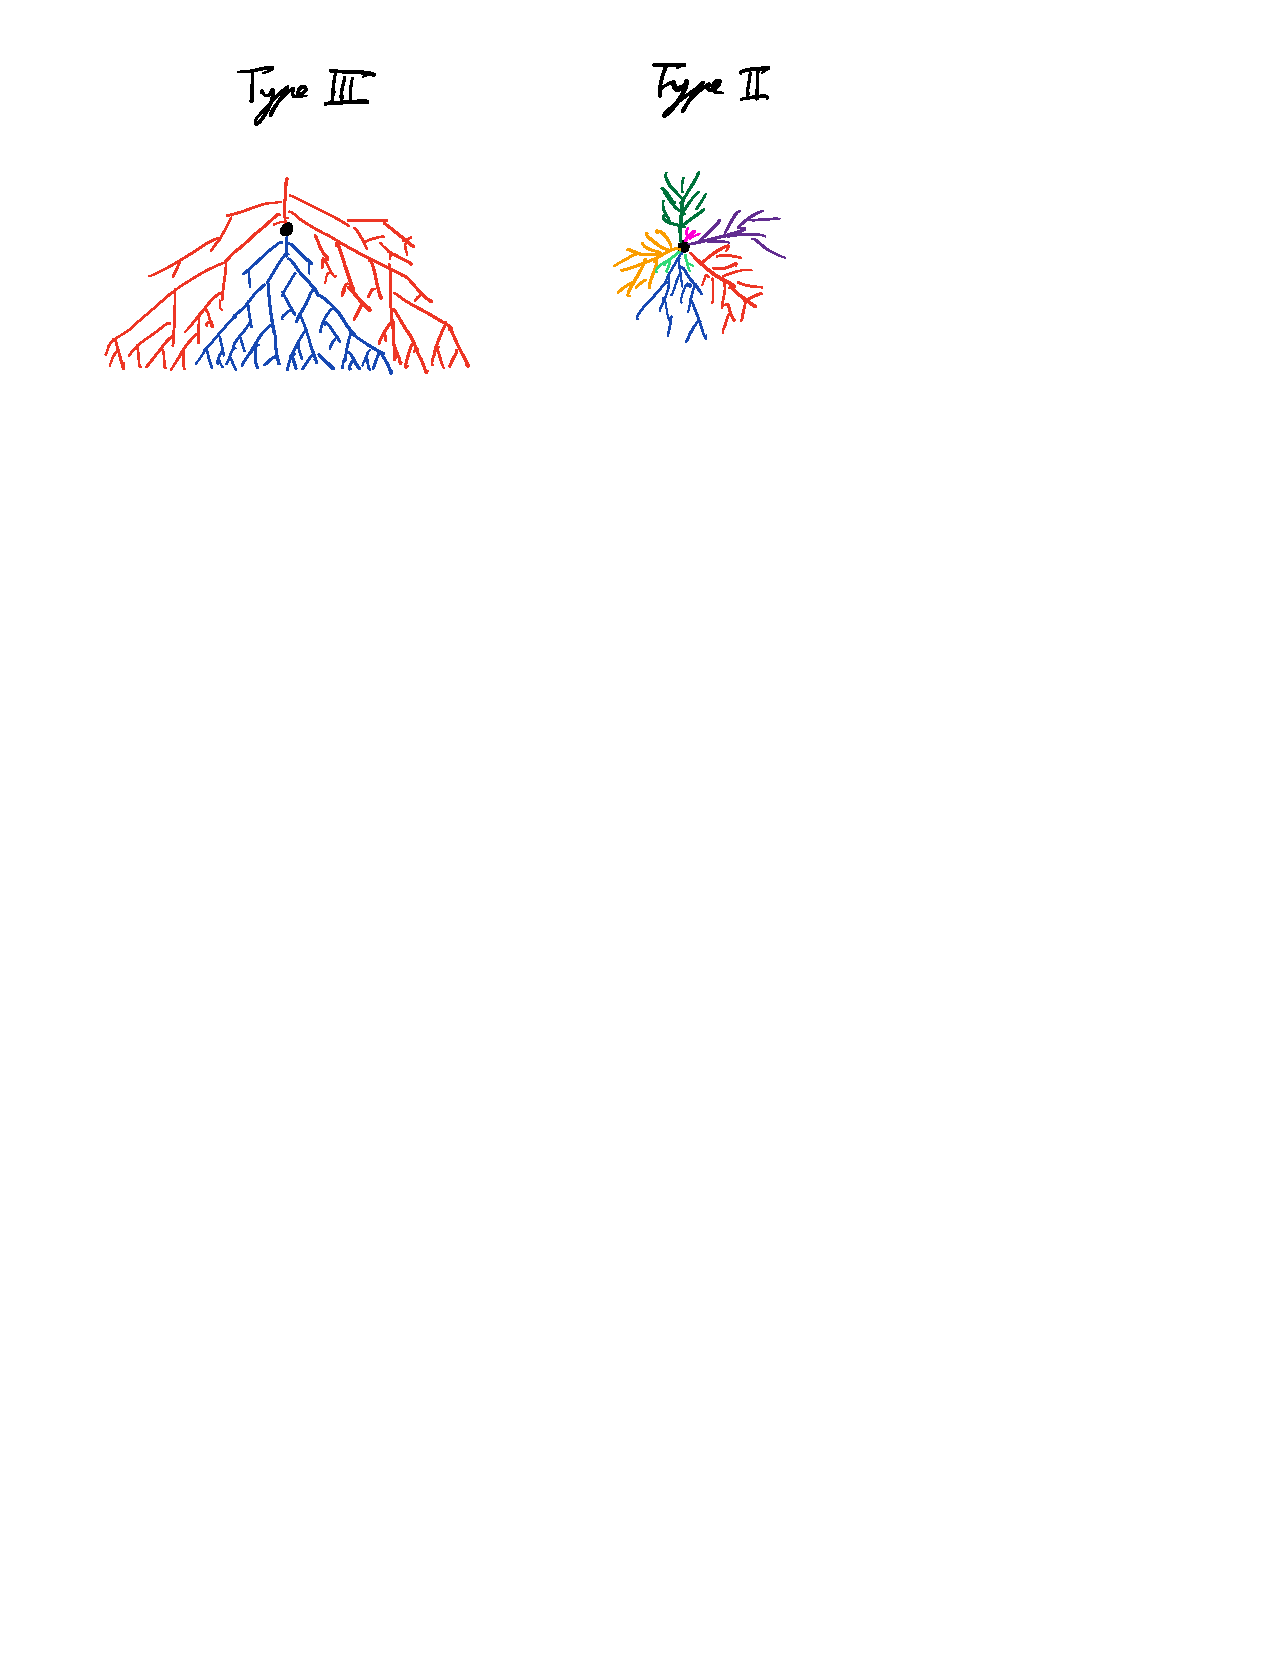
\includegraphics[width=0.7\textwidth]{figures/type2_type3.pdf}
	\caption{Recognizing type II and type III points by connected components/tangent directions}
	\label{fig:type2_type3}
\end{figure}
\todo{if there is time left, remake \cref{fig:type2_type3}}


The algebraic way to classify the points of $\aff_K^{1,\text{an}}$ is by using Abhyankar's inequality. 
It is a sort of trancendental analogue of \cref{prop:balancing_valuations}.
\begin{definition}
	Let $K \subset L$ be a non-archimedean field extension. 
	Then we define \[
		E_{\frac{L}{ K}} = \dim \frac{|L^{\times }|}{|K^{\times }|} \otimes_\Z \Q, \qquad F_{L / K} = \trdeg(\tilde L / \tilde K)
	.\] 
\end{definition}

\begin{theorem}[Abhyankar's inequality]
	Let $K \subset H \subset L$ be non-archimedean rings extending each others norm. Assume that $L$ is algebraic over $\hat{H}$ and that $H$ is of transcendence degree $n$ over $K$. Then \[
	E_{L / K} + F_{L / K}  \le n
	.\] 
\end{theorem}

If $x \in \aff_K^{1, \text{an}}$ is a norm (not a seminorm) then its residue field $\mathcal{H} (x)$ is a completion on $K(T)$ with respect to the norm induced by $x$. As $K(T)$ is of transcendence degree 1 Abhyankar's inequality states that \[
	E_{\mathcal{H} (x) / K} + F_{\mathcal{H} (x) / K} \le 1
.\] 
This also allows us to classify points, because either both $E_{\mathcal{H} (x) / K}, F_{\mathcal{H} (x) / K}$ are zero, or exactly one is $1$. 
\begin{proposition}[2.3.3.3 in \cite{temkinIntroductionBerkovichAnalytic2010}]\label{def:type_points_curve}
	Let $x \in \aff_K^{1, \text{an}}$, then 
	\begin{itemize}
		\item $x$ is of type I if $\mathcal{H} (x) = K$
		\item $x$ is of type II if $F_{\mathcal{H} (x) / K} = 1$ and $E_{\mathcal{H} (x) / K} = 0$. 
		\item $x$ is of type III if $F_{\mathcal{H} (x) / K} = 0$ and $E_{\mathcal{H} (x) / K} = 1$.
		\item $x$ is of type IV if $\mathcal{H} (x) \subsetneq K$ and  $F_{\mathcal{H} (x) / K} = E_{\mathcal{H} (x) / K} = 0$.
	\end{itemize}
\end{proposition}

\begin{remark}
	From now on we will use the classification of points from \cref{def:type_points_curve} as the definition of type 1-4 points.
\end{remark}


